\section{Ausblick}

    Neue Entwicklungsziele im Bereich des teil- und vollautonomen Fahrens stellen die elektronischen Fahrzeugsysteme vor neue Herausforderungen.\\
    Die selbstständige Durchführung der Fahraufgabe durch ein elektronisches System oder die aktive Unterstützung eines menschlichen Fahrzeugführers
    bedingt eine umfangreiche Erfassung und Auswertung von Fahrzeug- und Umgebungsdaten.\\
    Zu diesem Zweck müssen die bisherigen Sensorsysteme um weitere Systeme erweitert werden, die optische Umweltdaten über Kameras liefern, Umgebungsscans
    mittels Radar, Lidar oder Ultraschall durchführen. ~\cite{.BP06}\\

    Langfristig ist eines der Hauptziele der Industrie und des Rechtsgebers eine umfassende Vernetzung
    sämtlicher Entitäten, die am Verkehrsgeschehen aktiv oder passiv partizipieren zu einem intelligenten
    Transport System (ITS).\\
    Ein solches ITS soll den Teilnehmern innovative Dienste anbieten, mit dem Ziel das Verkehrsgeschehen
    effizient zu verwalten und zu koordinieren sowie zusätzliche Sicherheit für alle Beteiligten zu bieten. ~\cite{.BP04}\\

    Ein denkbares Szenario wäre zum Beispiel der aktive Austausch der Bewegungsdaten von Fahrzeugen im näherer Umfeld, um unnötige Brems-
    und Beschleunigungsvorgänge zu vermeiden, sowie die Übertragung von auslastungsspezifischen Geschwindigkeitsbegrenzungen von smarten Verkehrsschildern
    direkt an die Fahrzeuge. Auch die Kontaktlose Erfassung und Verrechnung von nutzungsabhängigen Gebühren wäre denkbar und ist bereits im Einsatz.\\

    Vorraussetzung, um ein solches ITS aufzubauen ist eine Standardisierung der verwendeten Protokolle und Technologien.
    Zu diesem Zweck gibt es auf nationaler und internationaler Ebene verschiedene Organisationen und Konsortien,
    die dieses Ziel seit mehreren Jahren aktiv vorantreiben.\\

    \subsection{Vehicle to Everyhing}
    Grundlage eines ITS ist die Vehicle to Everything Kommunikation, die das Fahrzeug als zentralen Punkt in den
    Kontext der unterschiedlichen Umgebungssysteme und Entitäten setzt. Dabei wird genauer unterschieden in die Teilbereiche:
    
    \subsubsection{Vehicle to Vehicle}
    V2V beschreibt die Vernetzung der Fahrzeuge untereinander mit dem Ziel relevante Fahrzeugdaten z.Bsp. über RIchtung und Geschwindigkeit auszutauschen.
    Desweiteren kann über V2V Kommunkikation weitere sicherheitsrelevante Nachrichten aus anderen Teilbereichen weitergeleitet werden.

    \subsubsection{Vehicle to Network}
    V2N beschreibt die Vernetzung des Fahrzeugs mit dem Telekommunikationsnetz und der Cloud. Dadurch können über den
    rein lokalen Kontext hinaus Ressourcen genutzt und Daten geteilt werden. Ein Beispiel für eine solche V2N ANwendung, die bereits
    im Einsatz ist, ist die Integration von cloudbasierten Navigationslösungen wie Google Maps in das Fahrzeug.
    
    \subsubsection{Vehicle to Infrastructure}
    V2I (alternative Bezeichnung: Vehicle to Roadside) beschreibt die Vernetzung des Fahrzeugs mit der umgebenden Verkehrsinfrastruktur. Zum Beispiel könnten smarte
    Mautstationen automatisiert Fahrzeuge erfassen und abrechnen oder smarte Ampelanlagen könnten die Ampelzyklen in Abhängigkeit
    der Anzahl der jeweils wartenden Fahrzeuge anpassen, um den Verkehrsfluss zu optimieren. 

    \subsubsection{Vehicle to Pedestrian}
    V2P beschreibt die Vernetzung des Fahrzeugs mit nichtmotorisierten Verkehrsteilnehmern. Ziel ist explizit der
    Schutz dieser Verkehrsteilnehmer, die bei Unfällen einen inherenten Nachteil haben. V2P ist dabei jedoch allgemeiner
    zu verstehen und umfasst neben der aktiven Kommunikation der Entitäten auch die Erfassung von Fussgängern über rein
    fahrzeugseitige Sensorsysteme.

    \subsubsection{Vehicle to Device}
    V2D beschreibt die Kommunikation des Fahrzeugs mit elektronischen Geräten. Aktuelle Einsatzgebiete für diese Form der Kommunikation
    sind mobile Applikationen für Smartphones, mit denen Fahrzeugfunktionen von außerhalb gesteuert werden können. Aktuelle Beispiele
    sind die App von Tesla, mit der Fahrzeuge ausgeparkt werden können oder eine neue Entwicklung von Volvo mit der physische Schlüsseltechnologie
    durch eine mobile Smartphoneapp zuerst ergänzt und später dann ersetzt werden soll. ~\cite{.BP05}
     
    \subsubsection{Vehicle to Grid}
    V2G bescchreibt die Vernetzung eines elektrischen Fahrzeuges mit dem Stromnetz mit dem Ziel die Batterien elektrischer Fahrzeuge als Speichermedien
    bidirektional in das Stromnetz zu integrieren.

    \subsection{ITS Technologie und Standardisierung}

    Aufgrund der heterogenen Landschaft an Fahrzeugherstellern, Infrastrukturbetreibern, Komponententechnologien und der Tatsache, dass die Möglichkeiten
    und Beschränkungen dieser neuartigen Technologien noch nicht ausgelotet sind wurde bereits früh ein konkreter Standardisierungs- und Normierungsbedarf erkannt.\\
    Aus dieser Erkenntnis heraus sind die wichtigsten Standardisierungsorganisationen ISO, CEN, ETSI und SAE dabei Referenzarchitekturen und Protokolle zu entwickeln, die
    die Grundlagen der Weiterentwicklung der Technologie bilden.\\
    Da die Lebens- und Nutzungsspanne von Fahrzeugen mittlerweile bei 15 Jahren angelangt ist und in naher Zukunft bis zu 20 Jahren prognostiziert werden während gleichzeitig die 
    Lebensspanne von Kommunikationsmedien immer kürzer wird liegt die grundlegende Schwierigkeit der Standardisierungsbemühungen darin, zukunftssichere Standards und Protkolle zu entwickeln,
     die von konkret verwendeten Kommunikationsmedien abstrahieren und sicherstellen, dass auch Fahrzeuge, die heute produziert werden auch in 20 Jahren noch ohne nennenswerte Einbussen der Funktionalität in die Verkehrssysteme
    integriert werden können. Da es für die Hersteller zudem nicht kosteneffizient ist, Fahrzeuge für regionale Märkte zu produzieren, müssen die Lösungen für ITS Systeme
    außerdem globale Einsatzmöglichkeiten bieten.\\
    Mit diesem Ziel hat die ISO mit der ISO 21217 2010 die CALM Referenzarchitektur formuliert, die eine schichtbasierte Lösung präsentiert, die die Applikationsschicht, in
    der die ITS Dienste bereitstellen und nutzen von der medienbasierten Kommunikation trennen.\\

    \begin{figure}
        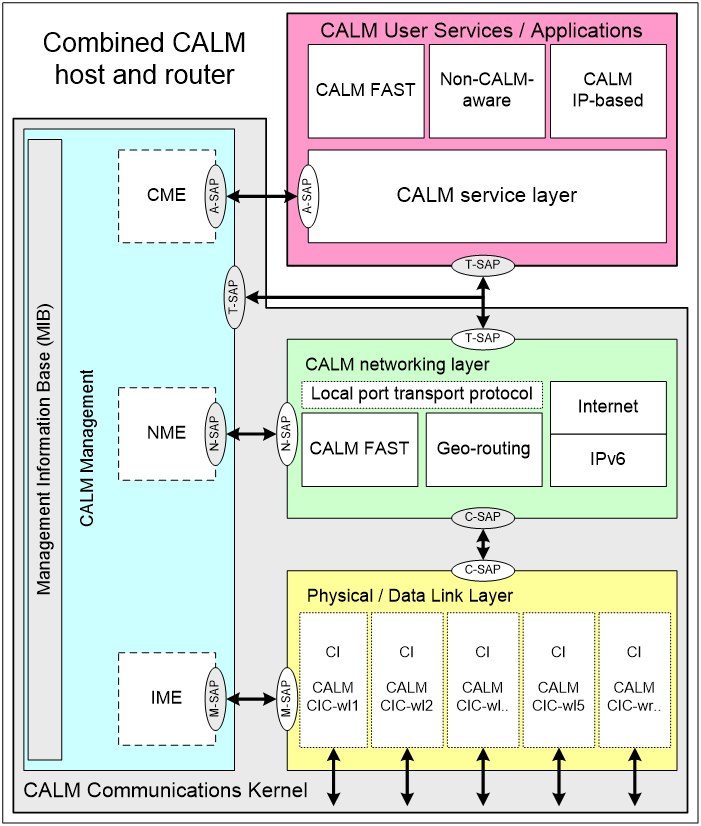
\includegraphics[width=\linewidth]{./images/BP/CALM.png}
        \caption{CALM Architektur ~\cite{.BP07}}
        \label{fig:CALM}
    \end{figure}

    Aufbauend auf dieser Referenzarchitektur existieren dann medienspezifische Konkretisierungen für die verschiedensten drahtlosen und drahtgebundenen Kommunikationsmedien.
    Die zwei wichtigsten Spezifikationen sind dabei die drahtlose Kommunikation auf der Grundlage von WLAN, die aufbauend auf der 802.11a Spezifikation im 802.11p Protokoll spezifiert ist 
    und das 3GPP Protokoll für eine drahtlose Kommunikation auf Basis von Mobilfunktechnologie.

    \subsubsection{IEEE 802.11p}
    Der IEEE 802.11p Standard, spezifiziert eine Erweiterung des IEEE 802.11 WLAN Standards, der die drahtlose Kommunikation in und mit Fahrzeugen ermöglicht.
    Diese Erweiterung war notwendig, da die Zeitspanne zur Kommunikation eines Fahrzeugs in Bewegung mit stationären Infrastrukturknoten oft nur sehr kurz ist, was prohibitiv für die komplexe Verbindungsaufbauphase
    bei klassischem WLAN ist. Daher ermöglicht 802.11p die direkte Kommunikation, ohne zuvor ein Basic Service Set zu etablieren.\\
    Da dies jedoch bedeutet dass die kommunizierenden Stationen nicht assoziert und nicht authentifiziert sind, müssen entsprechende Mechanismen in höheren Netzwerkschichten
    implementiert werden.\\
    IEEE 802.11p bildet den Grundstein für die Dedicated Short Range Communication Technik, in Europa als ITS-G5 bezeichnet. 
    
    Neben der drahtlosen Kommunikation auf Grundlage von WIFI, ist besonders für die Vernetzung über längere Entfernung die Verwendung bestehender oder zukünftiger Mobilfunksysteme möglich. 

   
    \subsection{Zusammenfassung und Fazit}
    Die Einbindung immer komplexerer elektronischer Systeme in Fahrzeugen hat die Entwicklung in den vergangenen
    20 Jahren rasant vorangetrieben. Zum Teil veraltete Standards müssen überdacht und modernisiert werden.\\
    Entwicklungen in der nahen Zukunft, die das Fahrzeug aus dem individuellen Kontext herauslösen und in ein holistisches volllvernetztes
    System integrieren mit dem Ziel erhöhter Sicherheit, verminderter Auswirkungen von Mobilität auf die Umwelt und der Entwicklung neuer Geschäftsmodelle
    und Mobilitätskonzepte stellen eine Herausforderung an die Standardisierungsorganisationen, da die Zusammenführung und Kooperation heterogener Systeme zu einem
    vereinheitlichten Gesamtsystem nur auf Grundlage zukunftsfähiger Standards möglich ist.\\
    
    Zudem bedeuten neue Antriebskonzepte wie Hybridmotoren oder rein elektrische Antriebe, dass sich die Landschaft elektronischer Fahrzeugsysteme
    weiter verändern wird. Viele Sensorsysteme zur Überwachung der mechanischen Motorkomponenten werden in elektrisch betriebenen Fahrzeugen obsolet, während
    neue komplexe Sensorsysteme, die teil- und vollautonomes Fahren ermöglichen, weiter Einzug in die Fahrzeuge halten.\\

    Daher kann und soll diese Ausarbeitung nur ein Ausgangspunkt für eine weitere Erschliessung des Themas in der gesamten Komplexität darstellen.
